\subsection{Quy trình đăng ký tài khoản}
Người dùng mở Đăng ký, nhập họ tên, username, email, số điện thoại và mật khẩu như Hình~\ref{fig:registration-reset}(a). Biểu mẫu chỉ gửi khi các trường và xác nhận mật khẩu hợp lệ.

Repository tạo danh tính Authentication rồi ghi \texttt{users/\{uid\}} và alias \texttt{usernames} trong transaction Firestore. Nếu ghi hồ sơ thất bại, hệ thống thử xóa danh tính để bù trừ vì hai dịch vụ không có transaction chung. Thành công thì mở giao diện GUEST.

\subsection{Quy trình đăng nhập và khôi phục mật khẩu}
Người dùng nhập email hoặc username và mật khẩu; username được tra cứu thành email trước khi xác thực. Ứng dụng kiểm tra hồ sơ ACTIVE để mở khu vực người thuê, Host hoặc Admin. Phiên hết hiệu lực, thiếu hồ sơ hoặc bị khóa đều được xử lý trước khi điều hướng.

Khi quên mật khẩu, người dùng nhập email ở Hình~\ref{fig:registration-reset}(b) và đặt lại qua liên kết Firebase. App chỉ thông báo kết quả gửi yêu cầu; người dùng đăng nhập lại sau khi hoàn tất.

\begin{figure}[H]\centering
\begin{minipage}[t]{0.27\linewidth}\centering\vspace{0pt}
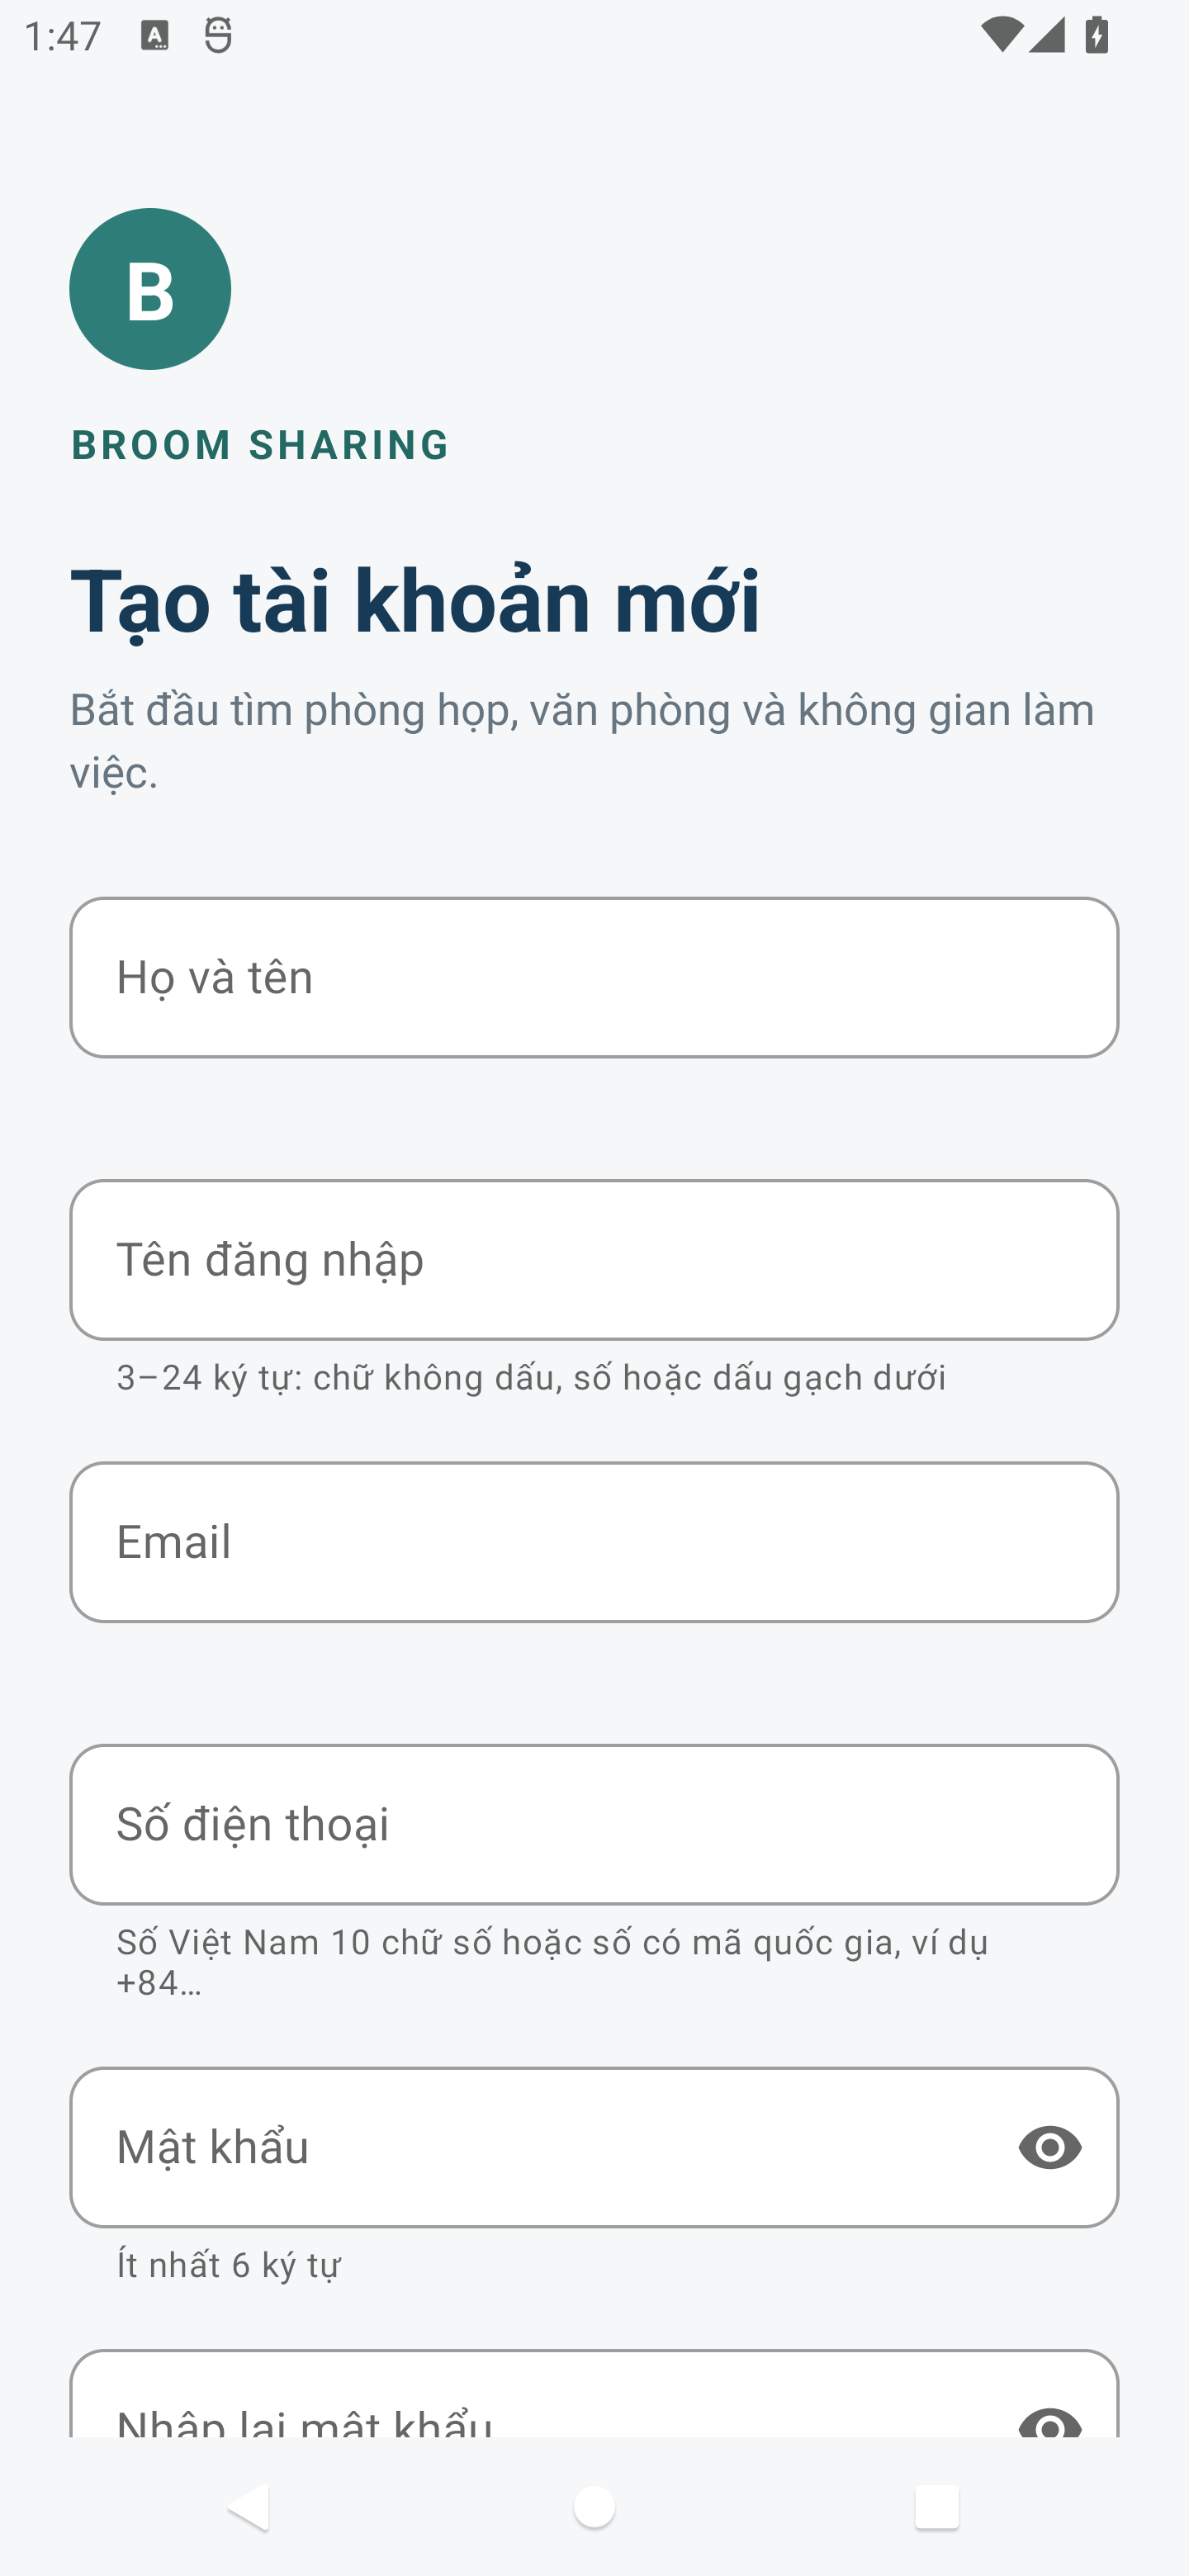
\includegraphics[height=0.35\textheight,width=\linewidth,keepaspectratio]{chapter5/final/register.png}\\[-1mm]
{\small (a) Nhập hồ sơ đăng ký}
\end{minipage}\hspace{0.05\linewidth}%
\begin{minipage}[t]{0.27\linewidth}\centering\vspace{0pt}
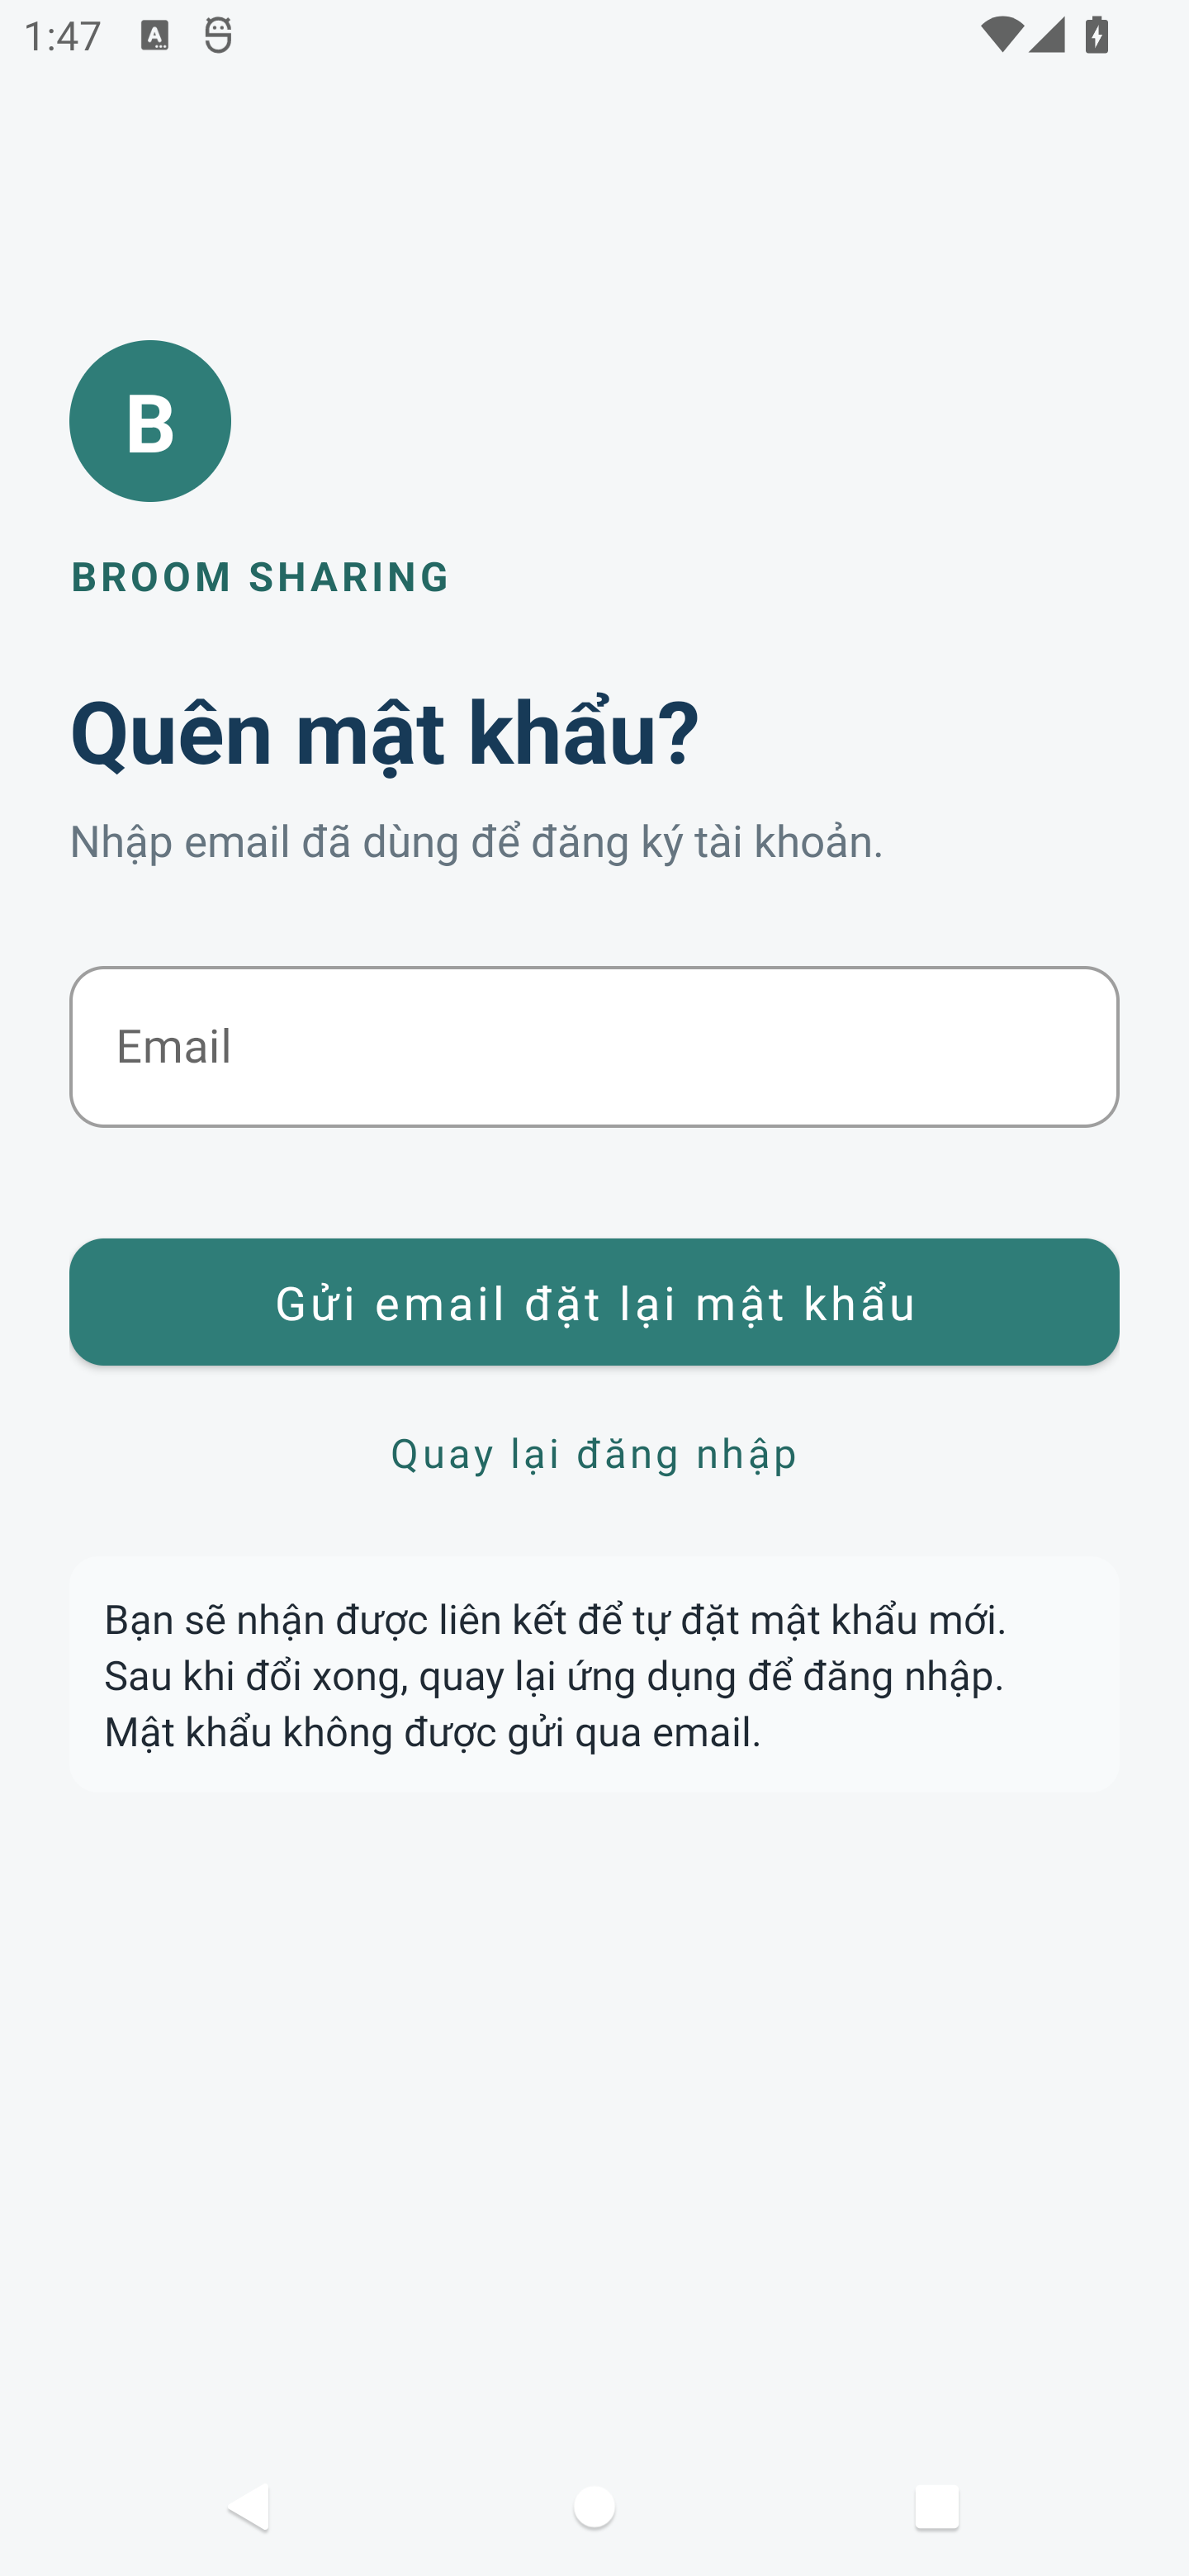
\includegraphics[height=0.35\textheight,width=\linewidth,keepaspectratio]{chapter5/final/reset-password.png}\\[-1mm]
{\small (b) Gửi yêu cầu đặt lại mật khẩu}
\end{minipage}
\caption{Các biểu mẫu đăng ký và khôi phục mật khẩu hiện thực}
\label{fig:registration-reset}
\end{figure}
